\documentclass{article}
\usepackage[usegeometry]{typearea}% load before geometry
\usepackage{geometry}
\usepackage{paralist}
\usepackage[T1]{fontenc}
\usepackage{reledmac}
\usepackage{changepage}
\usepackage{amsmath}
\usepackage{scalerel,amssymb}
\usepackage{colortbl}

\usepackage{pgfplots}
\usepackage{tikz}
\usetikzlibrary{positioning}
\usetikzlibrary{shapes.geometric, arrows}
\tikzstyle{arrow} = [thick,->,>=stealth]

%\usepackage{layout}
%\usepackage{showframe}

\graphicspath{ {./images/} }

\usepackage{fancyhdr}
\fancyhead[L]{
	\begin{tabular}{l}
		\LARGE \textbf{\textsc{Cryptographic Protocols}} \\
		\large Exercise 03
	\end{tabular}
}
\fancyhead[R]{
	\begin{tabular}{r}
		16-124-836 \\
		Marcel \textsc{Zauder}
	\end{tabular}
}
\renewcommand{\headrulewidth}{0.4pt}
\fancyfoot[C]{\thepage}
\renewcommand{\footrulewidth}{0.4pt}

\usepackage{hyperref}
\begin{document}
	\KOMAoptions{paper=landscape,DIV=last}
	\newgeometry{hmargin=2.5cm,bottom=25mm,height=150mm,includehead, textheight= 480pt}
	\fancyheadoffset{0pt}% recalculate headwidth for fancyhdr
	\pagestyle{fancy}
	\hfill
	
	\section*{3.1 Privacy in the Google-One-VPN}
	\begin{adjustwidth}{-6em}{}
		\begin{tabular}{lll}
			\begin{tabular}{l}
				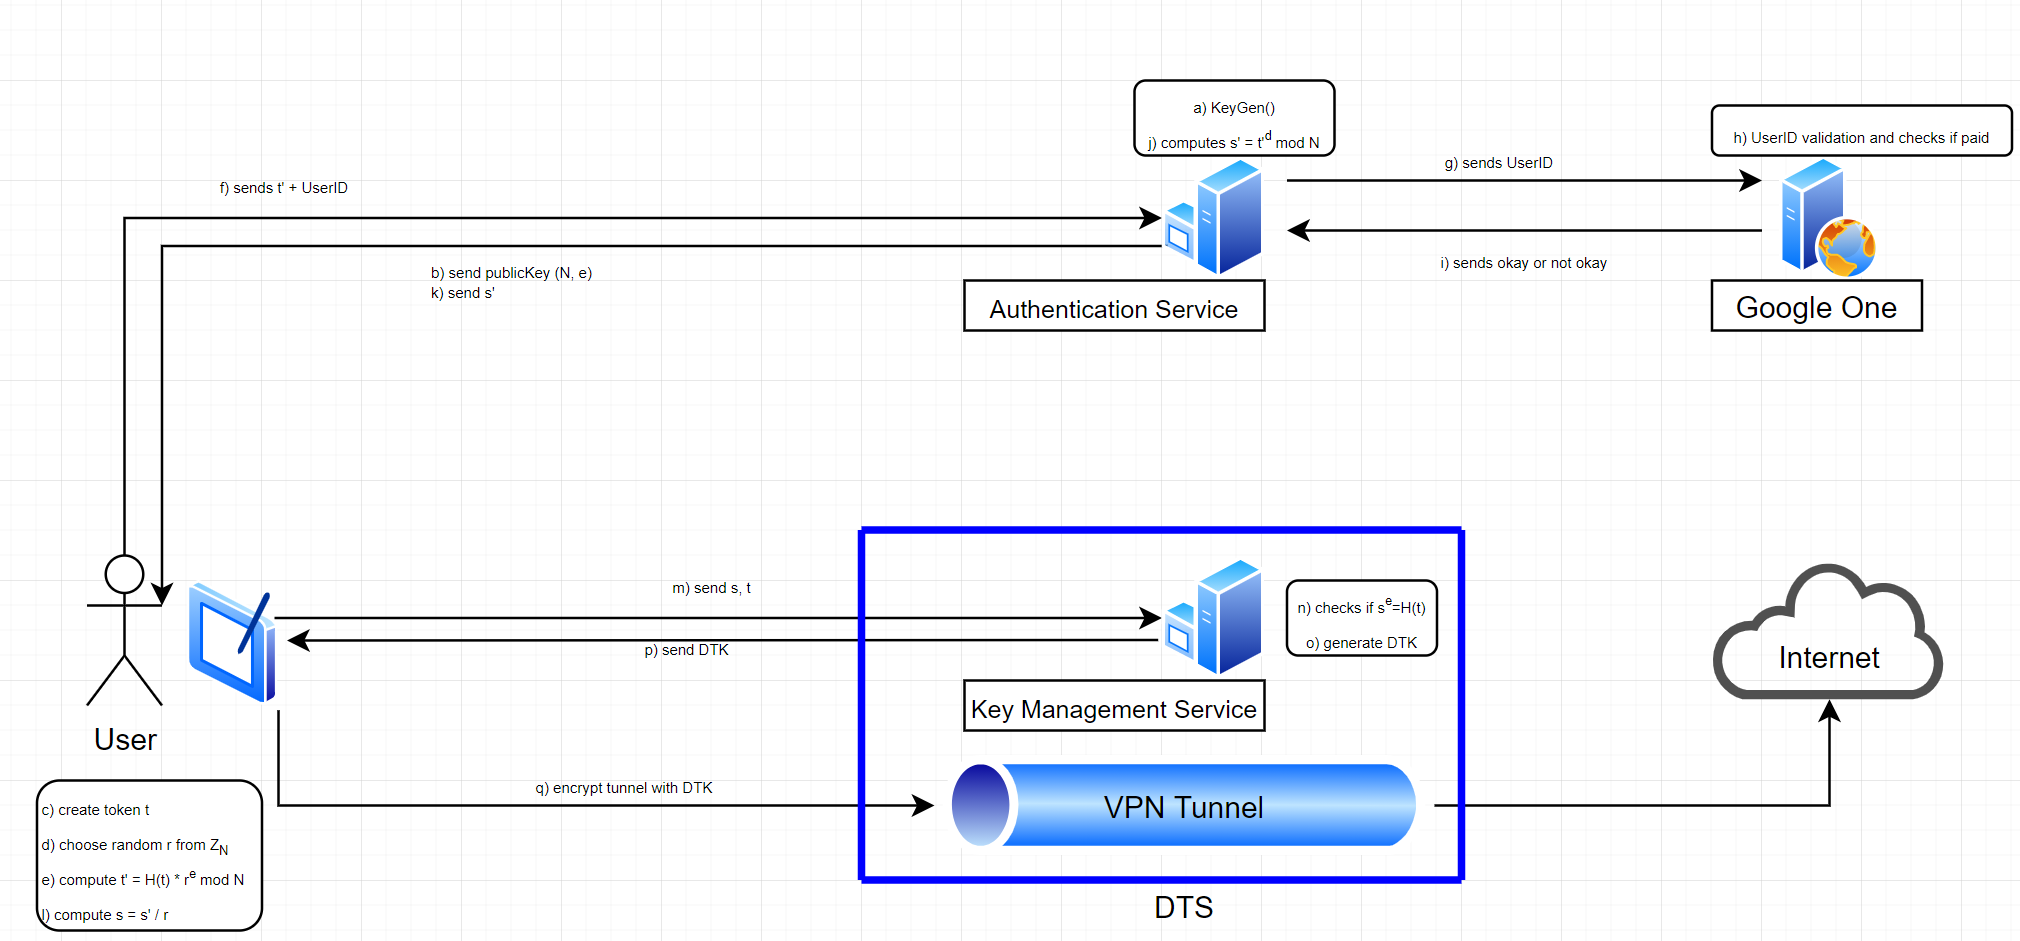
\includegraphics[scale=0.4]{GoogleOne_Diagram.png}
			\end{tabular}			
			&
			&
			\begin{tabular}{p{5cm}}
				The client gets the public key from the authentication service, with which he can encrypt his token, by using any random number that he has chosen and a full-domain-hash-function. This so blinded token is then sent to the Authentication Service together with the user's ID, which is needed for checking the validity of the acoount and whether the user has paid for the VPN or not. If everything is correct the AS sends a blinded signature back to the user, which can then be unblinded by him/her. With the unblinded signature and the created token the user can then ask the Key Management Service to create DTKs for him. This will happen after the KMS has checked the signature token pair for validity. After that the user can use the DTK to access the VPN. 
			\end{tabular}			 
		\end{tabular}
	\end{adjustwidth}
	\begin{adjustwidth}{2em}{2em}
		\textbf{Scope and lifetime of RSA public/private key:} \\
		The RSA key pairs can have a long lifetime because they are only used to encrypt a token from any user so it can be sent to the authentication service (AS). Therefore the public key has a global scope so anyone would be able to send his/her token to the AS. Only in the AS the UserData are checked for validity and the signature is created using the private key, therefore only itself knows about the private key and given there is no data leak it could be used indefinately (given DLP is hard), but in practice those would be recreated in a set time interval. \\ \\
		\textbf{Scope and lifetime of DTK:} \\
		DTK keys are like session keys, which are valid as long as the user is connected to the VPN, after logging out or a long time of inactivity these keys become invalid to ensure that a user cannot connect to the VPN with old DTKs (especially if their subscription already expired). Additionally those DTK keys should not be accessible from other clients.
	\end{adjustwidth}
\end{document}